\subsection{Matrix-Matrix Multiplication (HLPP)}

\from{HLPP begin}
We use matrix multiplication as an example to evaluate our allpairs skeleton implementations regarding programming effort and performance.


\subsubsection{Implementations of matrix multiplication}
We compare six different implementations of the matrix multiplication:
\begin{enumerate}
  \item the OpenCL implementation from~\cite{KiHw-10} without optimizations,
  \item the optimized OpenCL implementation from~\cite{KiHw-10} using GPU local memory,
  \item the optimized BLAS implementation by AMD~\cite{AMD-13} written in OpenCL,
  \item the optimized BLAS implementation by NVIDIA~\cite{NVIDIA-13} written in CUDA,
  \item the implementation using the generic allpairs skeleton,
  \item the implementation using the allpairs skeleton customized with zip-reduce.
\end{enumerate}

\paragraph{1. OpenCL implementation}
The kernel of the first, unoptimized OpenCL implementation from~\cite{KiHw-10} is shown in Listing~\ref{lst:naive_opencl}.
\begin{lstlisting}[%                                                             
caption={OpenCL kernel of the matrix multiplication without optimizations~\cite{KiHw-10}.},%
float=ht,%
numbers=left,%
label={lst:naive_opencl}]
__kernel void mm(__global float* A, __global float* B,
                 __global float* C, int m, int d, int n) {
  int row = get_global_id(0); int col = get_global_id(1);
  float sum = 0.0f;
  for (int k = 0; k < d; k++)
    sum += A[row * d + k] * B[k * n + col];
  C[row * n + col] = sum; }
\end{lstlisting}

\vspace{-.5em}
\paragraph{2. Optimized OpenCL implementations}
The kernel of the optimized OpenCL implementation from~\cite{KiHw-10} using local memory is shown in Listing~\ref{lst:local_mem_opencl}.
\begin{lstlisting}[%                                                             
caption={OpenCL kernel of the optimized matrix multiplication using local memory~\cite{KiHw-10}.},%
float=t,%
numbers=left,%
label={lst:local_mem_opencl}]
#define TILE_WIDTH 16
__kernel void mm(__global float* A, __global float* B,
                 __global float* C, int m, int d, int n) {
  __local float Al[TILE_WIDTH][TILE_WIDTH];
  __local float Bl[TILE_WIDTH][TILE_WIDTH];
  int   row = get_global_id(0); int   col = get_global_id(1);
  int l_row = get_local_id(0);  int l_col = get_local_id(1);
  float sum = 0.0f;
  for (int m = 0; m < d / TILE_WIDTH; ++m {
    Al[l_row][l_col] = A[row * d + (m * TILE_WIDTH + l_col)];
    Bl[l_row][l_col] = B[(m * TILE_WIDTH + l_row) * d + col];
    barrier(CLK_LOCAL_MEM_FENCE);
    for (int k = 0; k < TILE_WIDTH; k++)
      sum += Al[l_row][k] * Bl[k][l_col];
    barrier(CLK_LOCAL_MEM_FENCE); }
  C[row * n + col] = sum; }
\end{lstlisting}
Two fixed-sized arrays of local memory are allocated in lines 4 and 5.
Matrix multiplication is carried out in the loop starting in line 9.
In each iteration, data is loaded into the local memory (lines 10 and 11) before it is used in the computation in line 14.
Note that two synchronization barriers are required (lines 12 and 15) to ensure that the data is fully loaded into the local memory and that the data is not overwritten while other work-items are still using it.
Both OpenCL implementations 1. and 2. from~\cite{KiHw-10} are only capable of performing matrix multiplication for square matrices.

\vspace{-.5em}
\paragraph{3. BLAS implementation by AMD}
The implementation offered by AMD is called clBLAS, written in OpenCL and is part of their Accelerated Parallel Processing Math Libraries (APPML)~\cite{AMD-13}.

\vspace{-.5em}
\paragraph{4. BLAS implementation by NVIDIA}
The cuBLAS~\cite{NVIDIA-13} is implemented using CUDA and, therefore, can only be used on GPUs built by NVIDIA.

\vspace{-.5em}
\paragraph{5. Generic allpairs skeleton}
Listing~\ref{lst:basic_mm} in Section~\ref{sec:allpairs_skeleton} shows the implementation using the generic allpairs skeleton.

\vspace{-.5em}
\paragraph{6. Allpairs skeleton customized with zip-reduce}
Listing~\ref{lst:nested_allpairs} in Section~\ref{sec:opt_allpairs_skeleton} shows the implementation using the allpairs skeleton customized with zip-reduce.


\subsubsection{Programming effort}
As the simplest criterion for programming effort, we use the program size in lines of code (LoC).
Figure~\ref{fig:mat_mult_loc} shows the number of LoCs required for each of the six implementations.
Table~\ref{tab:mat_mult_loc} presents the detailed numbers.
We did not count those LoCs which are not relevant for parallelization and are similar in all six implementations, like initializing the input matrices with data and checking the result for correctness.
For every implementation, we distinguish between CPU code and GPU code.
For the OpenCL implementations, the GPU code is the kernel definition, as shown in Listing~\ref{lst:naive_opencl} and Listing~\ref{lst:local_mem_opencl};
the CPU code includes the initialization of OpenCL, memory allocations, explicit data transfer operations, and management of the execution of the kernel.
For the BLAS implementations, the CPU code contains the initialization of the corresponding BLAS library, memory allocations, as well as a library call for performing the matrix multiplication;
no definition of GPU code is necessary, as the GPU code is defined inside the library function calls.
For the generic allpairs skeleton (Listing~\ref{lst:basic_mm}), we count lines 1 -- 2 and 8 -- 10 as the CPU code, and the definition of the customizing function in lines 3 -- 7 as the GPU code.
For the allpairs skeleton customized with zip-reduce (Listing~\ref{lst:nested_allpairs}), lines 3 and 5 are the GPU code, while all other lines constitute the CPU code.

Both skeleton-based implementations are clearly the shortest, with 10 and 9 LoCs.
The next shortest implementation is the cuBLAS implementation with 65 LoCs -- 7 times longer than the SkelCL-based implementation.
The other three implementations require even 9 times more LoCs than the SkelCL-based implementation.

Besides their length, the other implementations require the application developer to perform many low-level, error-prone tasks, like dealing with pointers or offset calculations.
Furthermore, the skeleton-based implementations are more general, as they can be used for arbitrary allpairs computations, while the other four implementations perform matrix multiplication only.
\vspace{4em}

\begin{figure}[t]
  \centering
  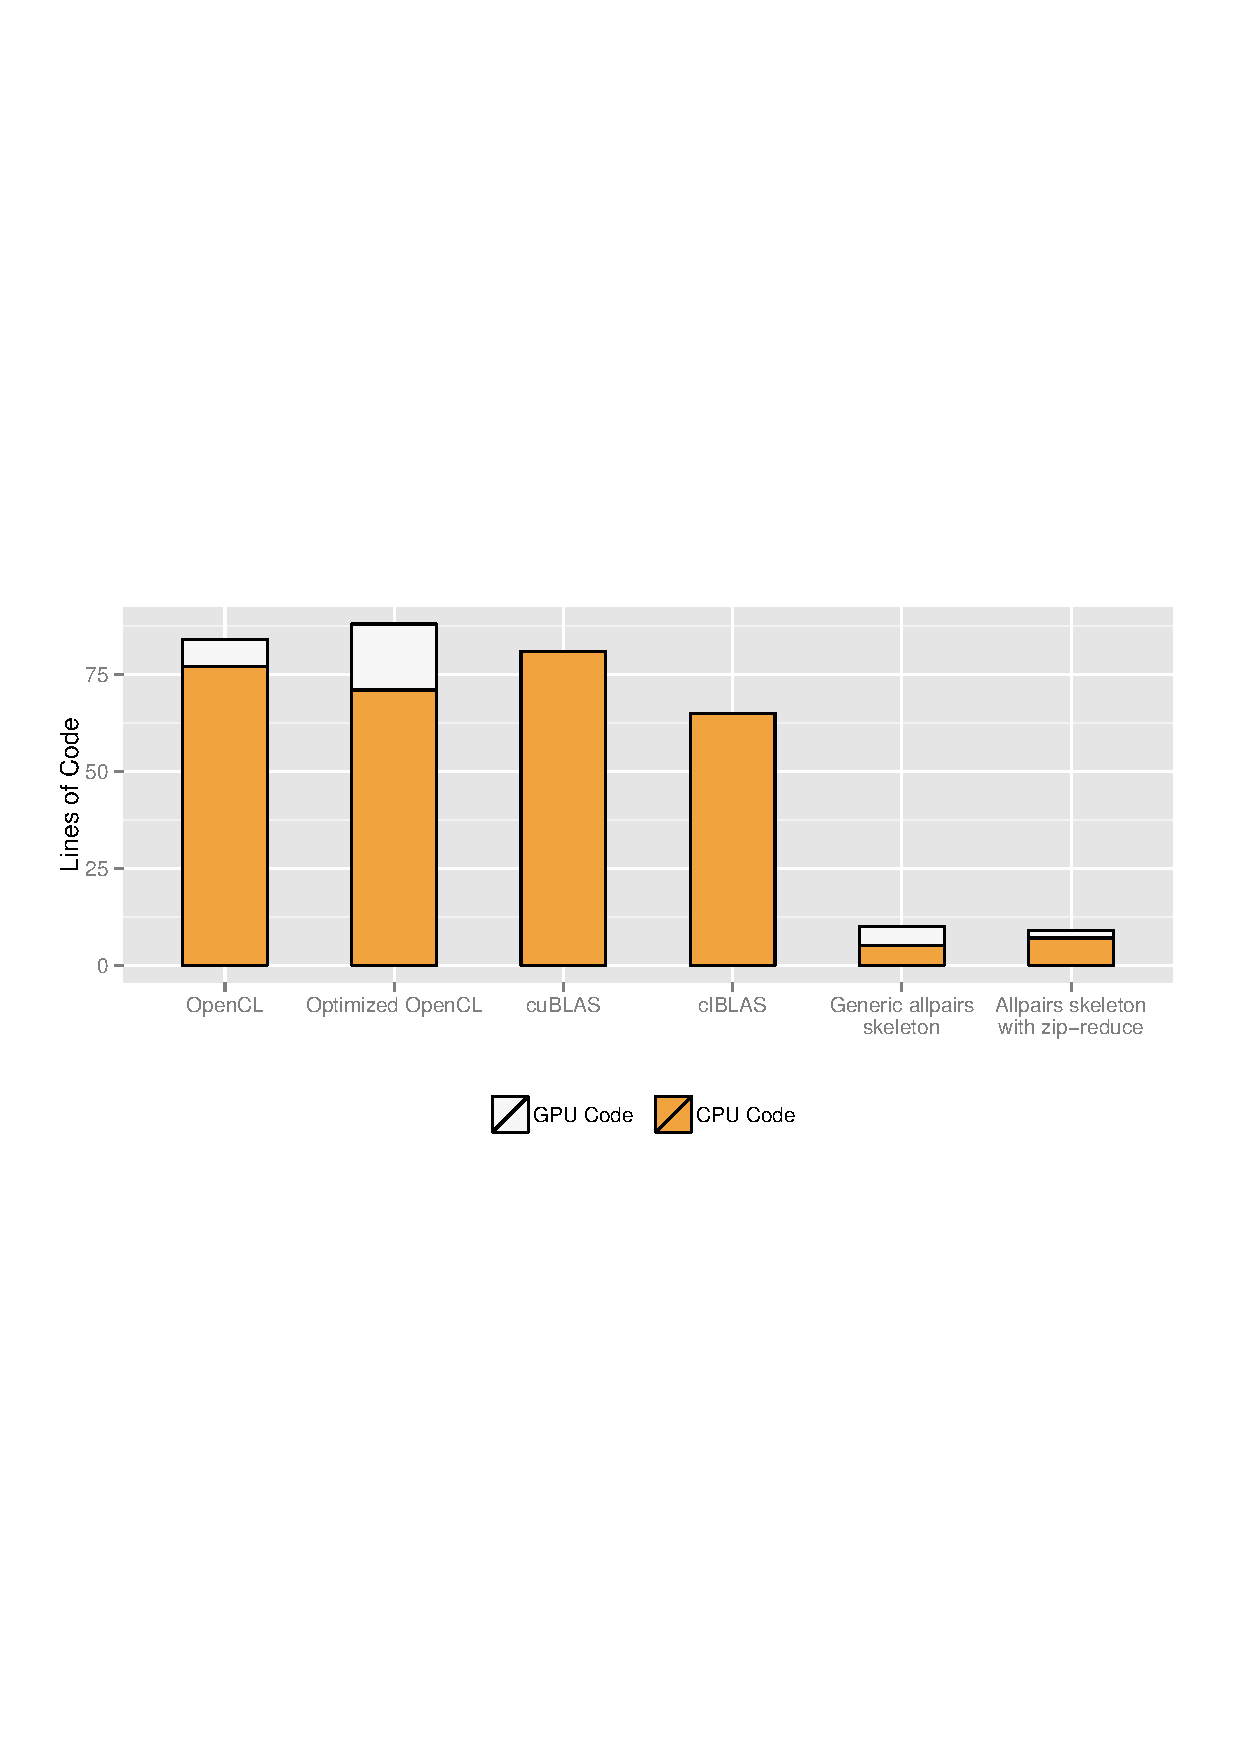
\includegraphics[width=0.9\textwidth]{HLPP/mat_mult_loc}
  \caption{Programming effort (Lines of Code) of all compared implementations.}
  \label{fig:mat_mult_loc}
\end{figure}
\begin{table}[b]
  \centering
  \begin{tabular}{lrr}
    \toprule
              & \multicolumn{2}{c}{Lines of Code} \\
    \cmidrule(r){2-3}
    Implementation & CPU & GPU \\
    \midrule
    OpenCL            & 77 &  7 \\
    Optimized OpenCL  & 71 & 17 \\
    cuBLAS            & 81 & -- \\
    clBLAS            & 65 & -- \\
    Generic allpairs  & \multirow{2}{*}{5} & \multirow{2}{*}{5}\\
    skeleton\\
    Allpairs skeleton & \multirow{2}{*}{7} & \multirow{2}{*}{2}\\
    with zip-reduce\\
    \bottomrule
  \end{tabular}
  \caption{Lines of Code of all compared implementations.}
  \label{tab:mat_mult_loc}
\end{table}

\subsubsection{Runtime experiments}
We performed our experiments with the six different implementations 1. -- 6. of matrix multiplication on two different computer systems with GPUs:
\begin{itemize}[leftmargin=50pt]
  \item[System A:] An NVIDIA S1070 equipped with four NVIDIA Tesla GPUs, each with 240 streaming processors and 4 GByte memory.
  \item[System B:] An AMD Radeon HD 6990 graphics card containing two GPUs, each with 1536 streaming processors and 1 GByte memory.
\end{itemize}

\begin{figure}[b]
  \centering
  \includegraphics[width=0.8\textwidth]{HLPP/mat_mult_sizes}
  \caption{Runtime of different matrix multiplication implementations on the NVIDIA system for different sizes for the matrices.}
  \label{fig:mat_mult_single}
\end{figure}
\begin{table}[b]
  \centering
  \begin{tabular}{lrrrrr}
    \toprule
              & \multicolumn{5}{c}{Runtimes in Seconds} \\
    \cmidrule(r){2-6}
    \multirow{2}{*}{Implementation} & $1024$ & $2048$ & $4096$ & $8192$ & $16384$ \\
                                    & $\times 1024$ & $\times 2048$ & $\times 4096$ & $\times 8192$ & $\times 16384$\\
    \midrule
    OpenCL            & 0.122 & 0.791 & 5.778 & 48.682 & 472.557 \\
    Optimized OpenCL  & 0.017 & 0.105 & 0.752 &  5.683 &  51.337 \\
    cuBLAS            & 0.012 & 0.059 & 0.387 &  2.863 &  22.067 \\
    clBLAS            & 0.061 & 0.246 & 1.564 & 11.615 &  90.705 \\
    Generic allpairs  & \multirow{2}{*}{0.121} & \multirow{2}{*}{0.792} & \multirow{2}{*}{5.782} & \multirow{2}{*}{48.645} & \multirow{2}{*}{471.235} \\
    skeleton\\
    Allpairs skeleton & \multirow{2}{*}{0.024} & \multirow{2}{*}{0.156} & \multirow{2}{*}{1.134} & \multirow{2}{*}{8.742} & \multirow{2}{*}{68.544} \\
    with zip-reduce\\
    \bottomrule
  \end{tabular}
  \caption{Detailed runtime results for all implementations on the NVIDIA system.}
  \label{tab:mat_mult_single}
\end{table}

In all our experiments, we include the time of data transfers to and from the GPU, i.\,e. the measured runtime consists of:
1) uploading the two input matrices to the GPU;
2) performing the actual matrix multiplication;
3) downloading the computed result matrix.

\paragraph{System A using one GPU.}
Figure~\ref{fig:mat_mult_single} shows the runtime in seconds of all six implementations for different sizes of the matrices (note that for readability reasons, all charts are scaled differently).
For detailed numbers, see Table~\ref{tab:mat_mult_single}.

Clearly, the naive OpenCL implementation and the implementation using the generic allpairs skeleton are the slowest, because both do not use the fast GPU local memory, in contrast to all other implementations.

The implementation using the allpairs skeleton customized with zip-reduce performs between 5.0 and 6.8 times faster than the implementation using the generic allpairs skeleton, but is 33\% slower on $16384\times 16384$ matrices than the optimized OpenCL implementation using local memory.
However, the latter implementation can only be used for square matrices and, therefore, omits many conditional statements and boundary checks.

\begin{figure}[b]
  \centering
  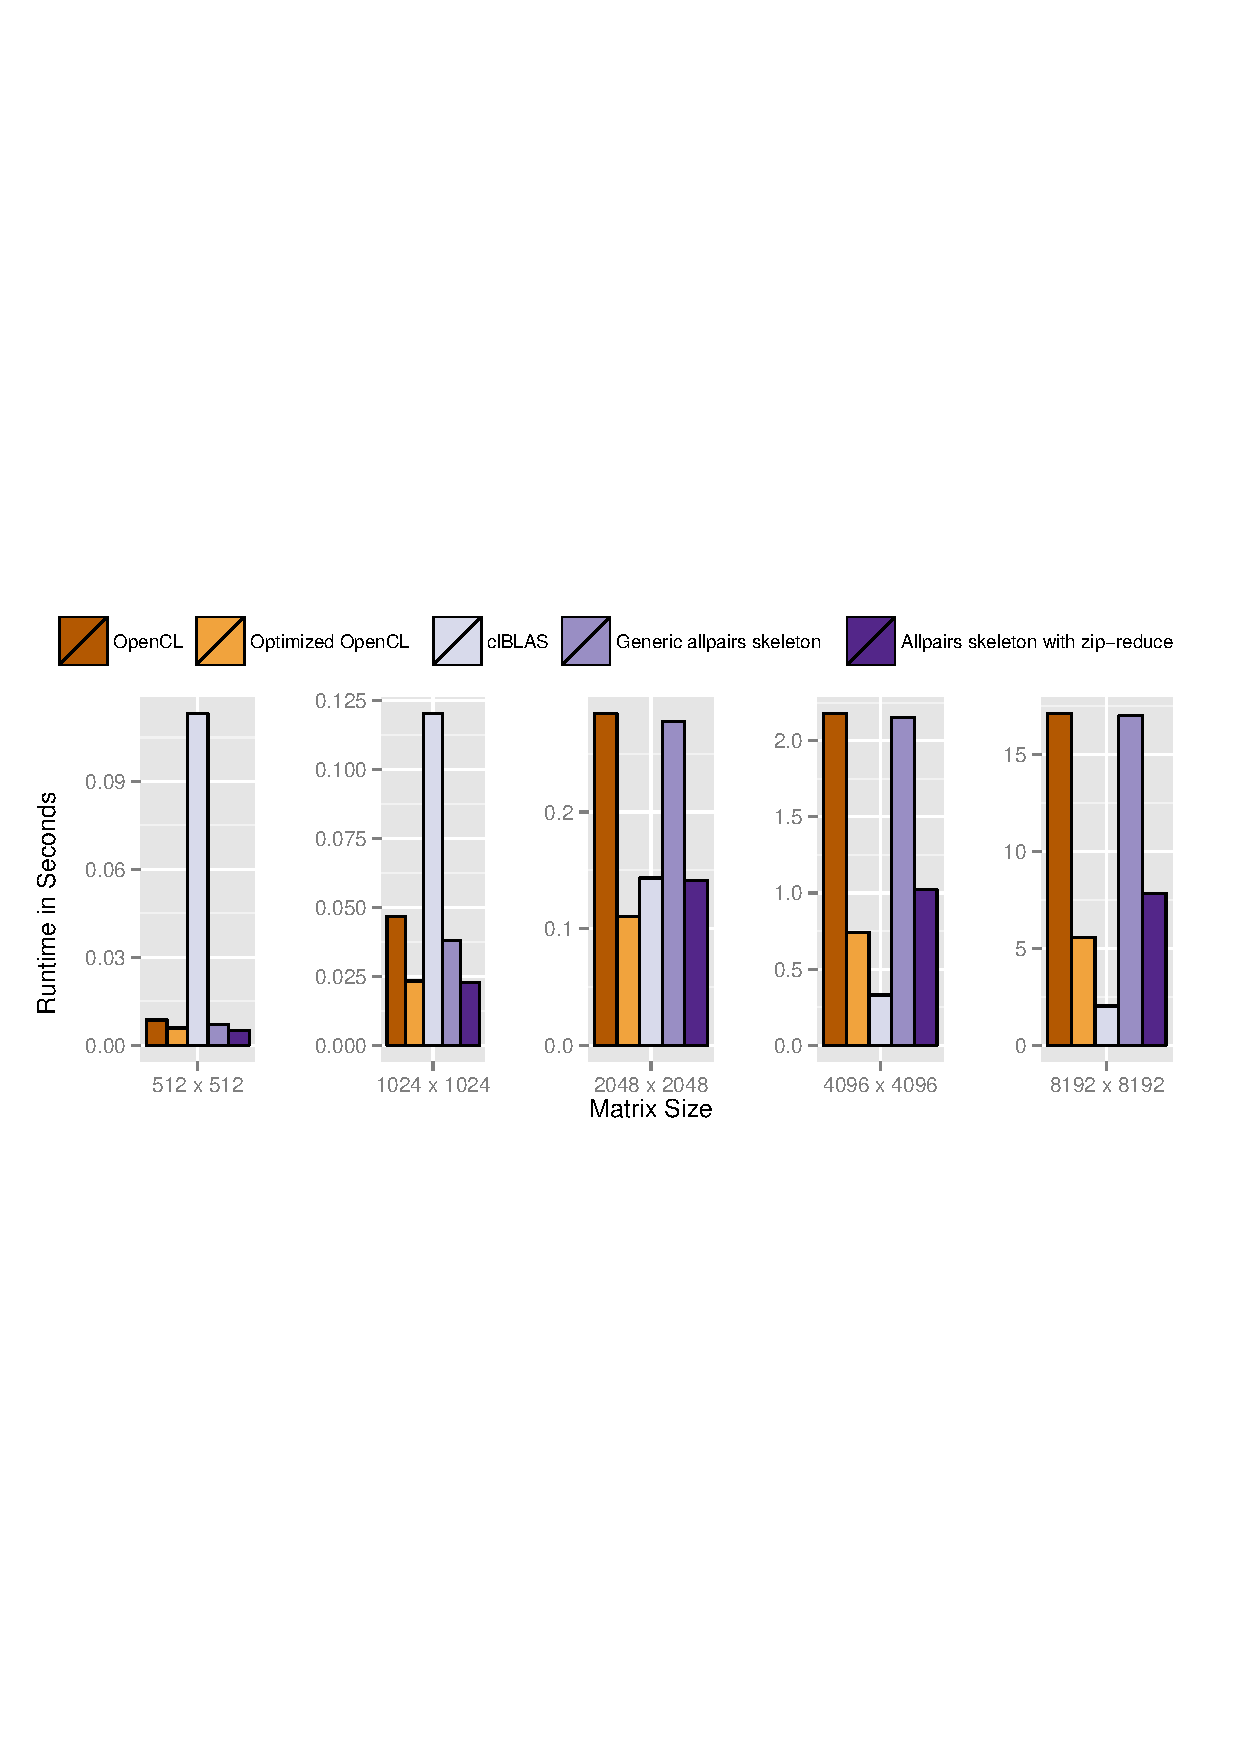
\includegraphics[width=0.8\textwidth]{HLPP/mat_mult_sizes_hd6990}
  \caption{Runtime of all compared implementations for a matrix multiplication on the AMD system using one GPU and different sizes for the matrices.}
  \label{fig:mat_mult_single_amd}
\end{figure}
\begin{table}[b]
  \centering
  \begin{tabular}{lrrrrr}
    \toprule
              & \multicolumn{5}{c}{Runtimes in Seconds} \\
    \cmidrule(r){2-6}
    \multirow{2}{*}{Implementation} & $512$ & $1024$ & $2048$ & $4096$ & $8192$ \\
                                    & $\times 512$ & $\times 1024$ & $\times 2048$ & $\times 4096$ & $\times 8192$ \\
    \midrule
    OpenCL            & 0.008 & 0.046 & 0.284 & 2.178 & 17.098 \\
    Optimized OpenCL  & 0.006 & 0.023 & 0.111 & 0.743 &  5.569 \\
    clBLAS            & 0.113 & 0.120 & 0.143 & 0.329 &  2.029 \\
    Generic allpairs  & \multirow{2}{*}{0.007} & \multirow{2}{*}{0.038} & \multirow{2}{*}{0.278} & \multirow{2}{*}{2.151} & \multirow{2}{*}{16.983} \\
    skeleton\\
    Allpairs skeleton & \multirow{2}{*}{0.005} & \multirow{2}{*}{0.023} & \multirow{2}{*}{0.141} & \multirow{2}{*}{1.025} & \multirow{2}{*}{7.842} \\
    with zip-reduce\\
    \bottomrule
  \end{tabular}
  \caption{Detailed runtime results for all implementations on the AMD system.}
  \label{tab:mat_mult_single_amd}
\end{table}

Not surprisingly, cuBLAS by NVIDIA is the fastest of all implementations, as it is highly tuned specifically for NVIDIA GPUs using CUDA.
The clBLAS implementation by AMD using OpenCL performs not as well:
presumably, it is optimized for AMD GPUs and performs poorly on other hardware.
Our optimized allpairs skeleton implementation outperforms the clBLAS implementation for all matrix sizes tested.

\paragraph{System B using one GPU.}
Figure~\ref{fig:mat_mult_single_amd} shows the runtime in seconds for five of the six implementations for different sizes of the matrices.
Detailed numbers can be found in Table~\ref{tab:mat_mult_single_amd}.
We could not use the NVIDIA-specific cuBLAS implementation as it does not work on the AMD GPU.

For bigger matrices, the slowest implementations are, again, the unoptimized OpenCL implementation and the implementation using the generic allpairs skeleton.

The optimized OpenCL implementation and the allpairs skeleton customized with zip-reduce perform similarly.
For matrices of size $8192\times 8192$, the optimized OpenCL implementation is about 30\% faster.

The clBLAS implementation performs very poorly for small matrices, but is clearly the fastest implementation for bigger matrices.
Similar to the cuBLAS implementation on the NVIDIA hardware, it is not surprising that the implementation by AMD performs very well on their own hardware.


\begin{figure}[b]
  \centering
  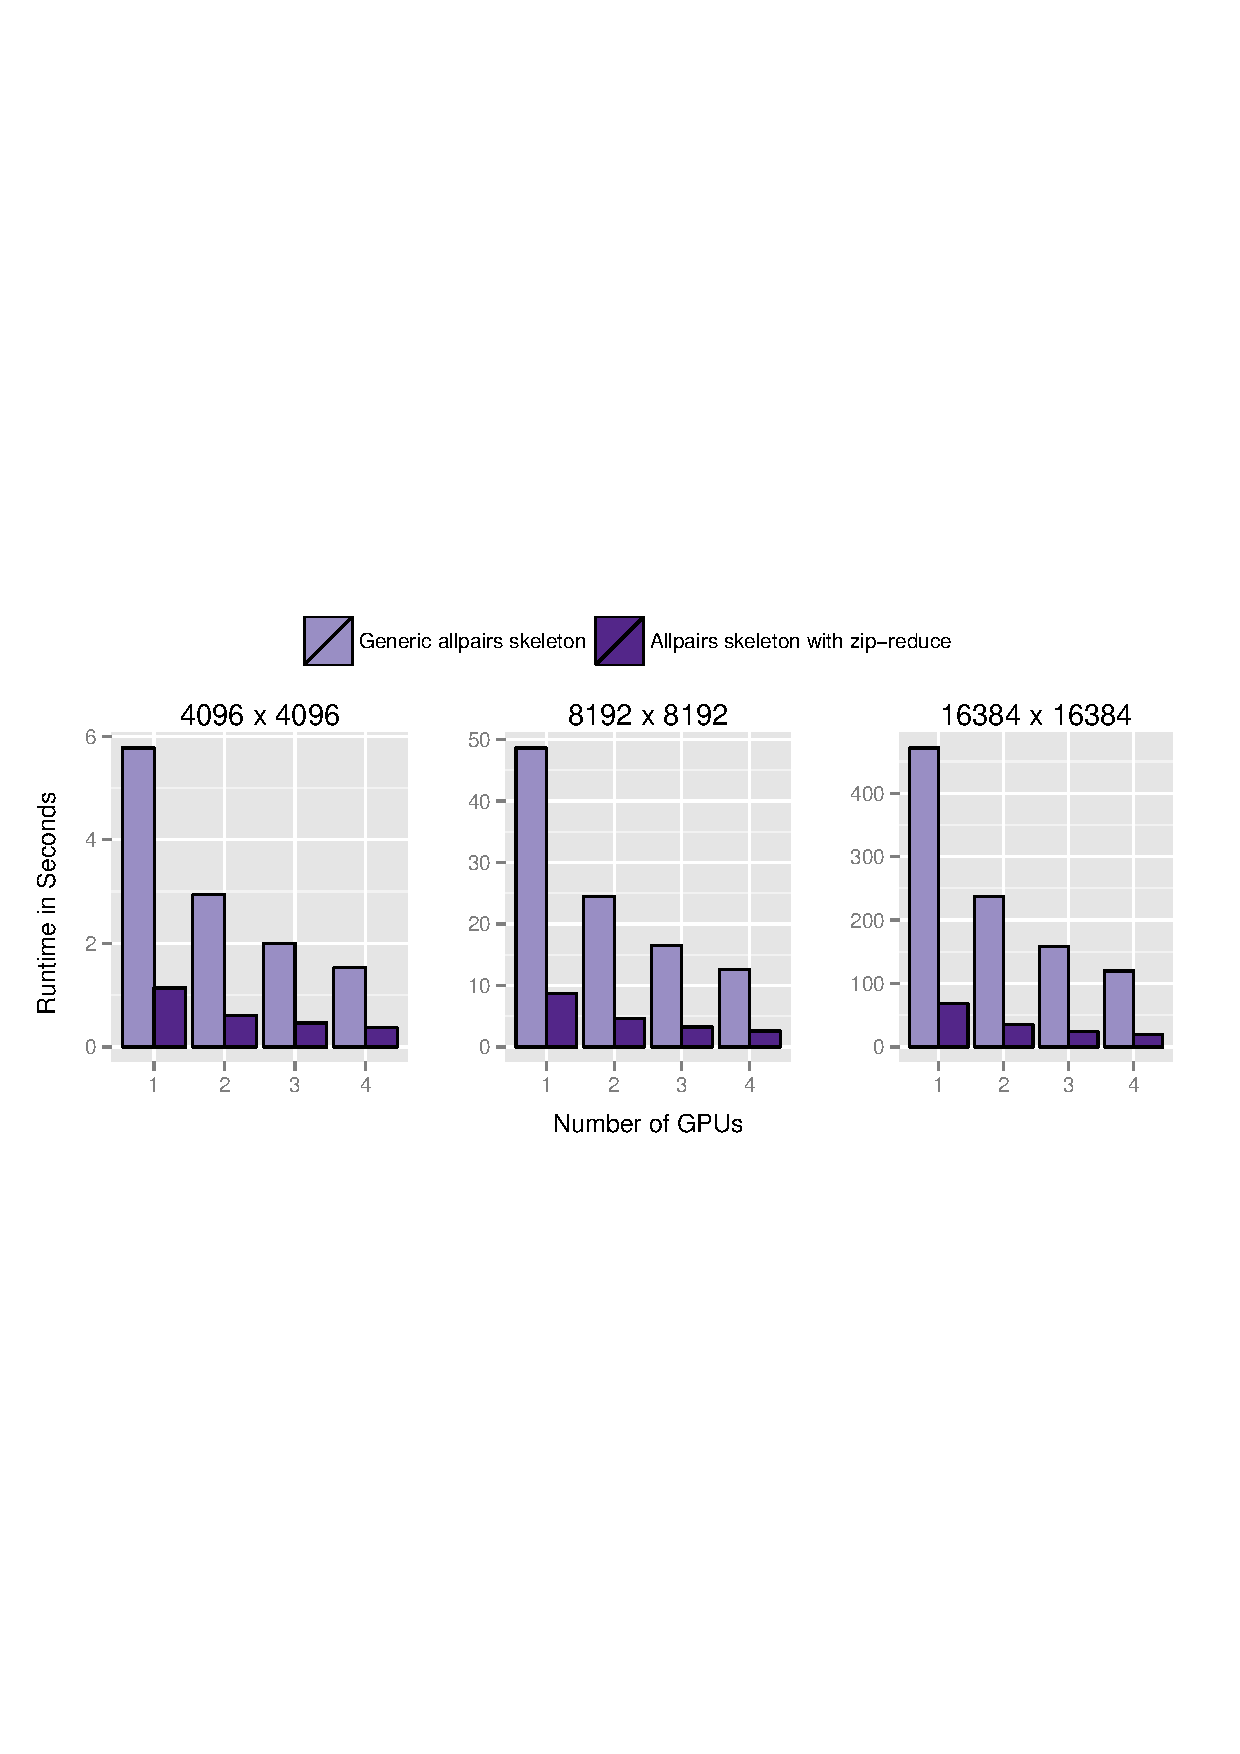
\includegraphics[width=0.8\textwidth]{HLPP/mat_mult_devices}
  \caption{Runtime of the allpairs based implementations using multiple GPUs.}
  \label{fig:mat_mult_devices}
\end{figure}
\begin{table}[b]
  \centering
  \begin{tabular}{llrrrcr}
    \toprule
              & & \multicolumn{3}{c}{Runtimes in Seconds} & & GFlops\\
    \cmidrule(r){3-5}
    \cmidrule(r){7-7}
    \multirow{2}{*}{Implementation}
     & Number    & $4096$ & $8192$ & $16384$ & & $16384$\\
     & of GPUs   & $\times 4096$ & $\times 8192$ & $ \times 16384$ & & $ \times 16384$\\
    \midrule
    \multirow{4}{*}{\parbox[t]{2.3cm}{Generic allpairs\\ skeleton}}
     & 1 GPU  & 5.772 & 48.645 & 471.328 &&  18.72\\
     & 2 GPUs & 2.940 & 24.495 & 236.628 &&  37.43\\
     & 3 GPUs & 2.000 & 16.532 & 158.611 &&  56.17\\
     & 4 GPUs & 1.527 & 12.540 & 119.786 &&  74.90\\[.5em]
    \multirow{4}{*}{\parbox[t]{2.3cm}{Allpairs skeleton\\ with zip-reduce}}
     & 1 GPU  & 1.137 &  8.740 &  68.573 && 130.93\\
     & 2 GPUs & 0.613 &  4.588 &  35.294 && 262.18\\
     & 3 GPUs & 0.461 &  3.254 &  24.447 && 392.87\\
     & 4 GPUs & 0.368 &  2.602 &  19.198 && 523.91\\
    \bottomrule
  \end{tabular}
  \caption{Detailed runtime of the allpairs based implementations using multiple GPUs.
    For the matrices of size $16384\times 16384$ the results are also shown in GFlops.}
  \label{tab:mat_mult_devices}
\end{table}

\paragraph{System A using multiple GPUs.}
Figure~\ref{fig:mat_mult_devices} shows the runtime behavior for both allpairs skeleton-based implementations when using up to four GPUs of our multi-GPU system.
The other four implementations are not able to handle multiple GPUs and would have to be specially rewritten for such systems.
We observe a good scalability of our skeleton-based implementations, achieving speedups between 3.09 and 3.93 when using four GPUs.
Detailed numbers can be found in Table~\ref{tab:mat_mult_devices}.
For the matrices of size $16384\times 16384$, performance is also provided in GFlops;
to compute this value we excluded the data-transfer time (as usually done in related work) for a better comparison.
\from{HLPP end}

